\documentclass[9pt, c, compress]{beamer}	% Compile at least twice!
% \setbeamertemplate{navigation symbols}{}
\usetheme{Hannover}
\usepackage{ctex}
\useinnertheme{rectangles}
% \useoutertheme[title,section,subsection=true]{smoothbars}
% \usecolortheme{beaver}
\usecolortheme{seahorse}
\usecolortheme{orchid}
% \useinnertheme{default}
% \useoutertheme{default}

% -------------------
% Packages
% -------------------
\usepackage{
  amsmath,			% Math Environments
  amssymb,			% Extended Symbols
  enumerate,		    % Enumerate Environments
  graphicx,			% Include Images
  lastpage,			% Reference Lastpage
  multicol,			% Use Multi-columns
  multirow,			% Use Multi-rows
  pifont,			    % For Checkmarks
  stmaryrd,			% For brackets
  xcolor % For define of variout colors
}
\usepackage[english]{babel}

% -------------------
% Fonts & Layout
% -------------------
% \useinnertheme{default}
% \usefonttheme{serif}
\usefonttheme{structurebold}
\usepackage{mathptmx}
\usepackage{helvet}
\usepackage{palatino}
\setbeamerfont{title like}{shape=\scshape}
\setbeamerfont{frametitle}{shape=\scshape}
\setbeamertemplate{itemize items}[rectangles]
\setbeamertemplate{enumerate items}[default]
\setbeamertemplate{footline}[split]
\setbeamertemplate{blocks}[rounded][shadow=true]



% -------------------
% Commands
% -------------------

% Special Characters
\newcommand{\N}{\mathbb{N}}
\newcommand{\Z}{\mathbb{Z}}
\newcommand{\Q}{\mathbb{Q}}
\newcommand{\R}{\mathbb{R}}
%\newcommand{\C}{\mathbb{C}}

% Math Operators
\DeclareMathOperator{\im}{im}
\DeclareMathOperator{\Span}{span}

% Special Commands
\newcommand{\pf}{\noindent\emph{Proof. }}
\newcommand{\ds}{\displaystyle}
\newcommand{\defeq}{\stackrel{\text{def}}{=}}
\newcommand{\ov}[1]{\overline{#1}}
\newcommand{\ma}[1]{\stackrel{#1}
{\longrightarrow}}
\newcommand{\twomatrix}[4]{\begin{pmatrix} #1 & #2 \\ #3 & #4 \end{pmatrix}}
\newcommand{\ft}[1]{\frametitle{\textcolor{white}{#1}}}


% -------------------
% Tikz & PGF
% -------------------
\usepackage{tikz}
\usepackage{tikz-cd}
% 公式字体
% \usepackage{newtxtext,newtxmath}
\usetikzlibrary{
  calc,
  decorations.pathmorphing,
  matrix,arrows,
  positioning,
  shapes.geometric
}
\usepackage{pgfplots}
\usepackage{hyperref}
\hypersetup{
    colorlinks=true,
    filecolor=blue,
    linkcolor=black,  
    urlcolor=purple,
    citecolor=cyan,
}
\usepackage{mathtools}
\usepackage{fontspec}
\usepackage{listings}
\usepackage{ulem}

\lstset{ %
  % backgroundcolor=\color{white},      % choose the background color
  basicstyle=\footnotesize\fontspec{Consolas},  % size of fonts used for the code
  columns=fullflexible,
  tabsize=4,
  breaklines=true,               % automatic line breaking only at whitespace
  captionpos=b,                  % sets the caption-position to bottom
  commentstyle=\color{gray},  % comment style
  escapeinside={\%*}{*)},        % if you want to add LaTeX within your code
  keywordstyle=\color{blue},     % keyword style
  stringstyle=\color{mymauve}\ttfamily,  % string literal style
  frame=shadowbox,
  rulesepcolor=\color{red!20!green!20!blue!20},
  breaklines = true,                  % 代码过长则换行
  numbers = left,                     % 行号在左侧显示
  % identifierstyle=\color{red},
  language=c++,
}
\pgfplotsset{compat=newest}


% -------------------
% Theorem Environments
% -------------------
\theoremstyle{plain}
\newtheorem{thm}{Theorem}[section]
\newtheorem{prop}{Proposition}[section]
\newtheorem{lem}{Lemma}[section]
\newtheorem{cor}{Corollary}[section]
\theoremstyle{definition}
\newtheorem{ex}{Example}[section]
\newtheorem{nex}{Non-Example}[section]
\newtheorem{dfn}{Definition}[section]
\theoremstyle{remark}
\newtheorem{rem}{Remark}[section] 
\numberwithin{equation}{section}


% -------------------
% Title Page
% -------------------
\title{数论基础}
\subtitle{ACM中的数学小知识}
\author[dcac]{陈德创 \\
Codeforces: \textcolor{purple}{\href{https://codeforces.com/profile/dcac}{dcac}}}
\date{\today} 


\logo{
\includegraphics[height=0.7cm]{logo_xdblue.pdf}}

% \setbeamercolor{titlelike}{bg=grey,fg=white}

\setbeamerfont{frametitle}{size=\huge}
\setbeamerfont{framesubtitle}{size=\large}
\setbeamerfont{frametitle}{series=\bfseries}

% \setbeamertemplate{frametitle}
% {\begin{beamercolorbox}[wd=\paperwidth]{frametitle}
%     
\includegraphics[height=0.7cm]{logo_xdblue.pdf}
%     % \hfill
%     \insertframetitle
%   \end{beamercolorbox}
% }

%% 在每个章节的前面显示目录提示
\AtBeginSection[]
{
	\begin{frame}
		% \frametitle{Outline}
    \begin{multicols}{2}
      \tableofcontents[currentsection]
      \addtocounter{framenumber}{-1}
    \end{multicols}
	\end{frame}
}



% -------------------
% Content
% -------------------
\begin{document}

% Title Page
\begin{frame}
\insertlogo
\titlepage
\end{frame}

% \begin{frame}
% \tableofcontents
% \end{frame}

% 概述
\section{概述}
% My Motivation 
\subsection{简介}
\begin{frame}{简介}
主要讲什么?
\begin{itemize}
  \item ACM中的基础数学小知识
\end{itemize}
\pause
有啥用?
\begin{itemize}
  \item 单独的题目考察
  \item 一些题目解答的必备前提
  \item 玩
\end{itemize}
\end{frame}


\subsection{符号约定}
% Definitions & Examples
\begin{frame}{符号约定}
\begin{enumerate}
  \item $x|y$:x整除y,即x是y的因数,y是x的倍数
  \item $x\mod y$:x除以y的得到的余数
  \item $x\equiv y \pmod{M}$:x同余y(在模M的意义下)
  \item $\gcd(x,y)$:x和y的最大公约数,简写作$(x,y)$
  \item $\text{lcm}(x,y)$:x和y的最小公倍数,简写作$[x,y]$
  \item $\lfloor x \rfloor$:下取整
  \item $\lceil x \rceil$:上取整
  \item $[\text{命题}P]$:当命题$P$为真时值为1,否则为0
  \item $\sum$:求和,如$\sum\limits_{i=1}^{n}f(i)$,$\sum\limits_{1\leq i\leq n, i\in P}f(i)$
\end{enumerate}
\end{frame}

% 整除与同余
\section{整除与同余}
\subsection{整除}
\begin{frame}{整除基本性质}
\textbf{整除的定义}:若整数$a$除以非零整数$b$,商为整数且余数为零,即$a$能被$b$整除,记做$b|a$,读作:$b$整除$a$或$a$能被$b$整除。$a$叫做$b$的倍数,$b$叫做$a$的约数,或称为因数。
\pause
\begin{itemize}
  \item 若$a|c,b|c$,则$a|(b\pm c)$
  \item 若$a|b$,则对任意的$c(c\neq 0)$,有$a|bc$
  \item 若$a|b$,且$b|c$,则$a|c$
  \item 若$a|bc$,且$(a,c)=1$,则$a|b$
  \item 若$c|a$,且$c|b$,则对于任意整数$m,n$,有$c|(ma+nb)$
  \item 若$a|c,b|c$,且$(a,b)=1$,则$ab|c$
  \item \textbf{带余除法定理}: $\forall a,b>0, a,b\in \N$,$\exists$唯一的数对$q,r$,使$a=bq+r,(0\leq r<b)$。
\end{itemize}
\end{frame}


\subsection{同余}
\begin{frame}{同余基本性质}
\begin{itemize}
  \item 若$a\equiv b\pmod{m},c\equiv d\pmod{m}$,\\则$a\pm b\equiv c\pm d\pmod{m}$
  \item 若$a\equiv b\pmod{m},c\equiv d\pmod{m}$,\\则$a\times b\equiv c\times d\pmod{m}$ \pause
  \item 证明基本思路:$a=k_1m+b,c=k_2m+b$ \pause
  \item 基本用法:求模运算下求解问题(避免大数运算)、快速幂 \pause
  \item \textbf{注意}:除法不满足以上的性质
\end{itemize}
\end{frame}

\subsection{快速幂}
\begin{frame}[fragile]{快速幂}
  求解:$a^b\equiv x\pmod{m},(a,b\leq 1e9)$
  \vspace{0.5cm}
  \pause
\begin{itemize}
  \item 朴素求法:
\begin{lstlisting}
inline ll mpow(ll a, ll b, ll m) {
  ll res = 1;
  for (int i = 1; i <= b; ++i) 
    res = res * a % m;
  return res;
}
\end{lstlisting}
  \item 时间复杂度:$O(b)$
\end{itemize}
\end{frame}


\begin{frame}[fragile]{快速幂}
  求解:$a^b\equiv x\pmod{m},(a,b\leq 1e9)$
  \vspace{0.5cm}
\begin{itemize}
  \item 快速幂
\begin{lstlisting}
  inline ll mpow(ll a, ll b, ll m) {
    ll res = 1;
    while(b) {
      if (b & 1) res = res * a % m;
      a = a * a % m;
      b >>= 1;
    }
    return res;
  }
\end{lstlisting}
  \item 时间复杂度:$O(\log{b})$
\end{itemize}
\end{frame}

% 素数
\section{素数}
\subsection{素数}
\begin{frame}{素数基础}
  \textbf{定义}:只能被1和自身整除的数称为素数,又称为质数
  \begin{itemize}
    \item 1既不是素数,也不是合数
    \item 2是最小的素数,也是唯一的偶素数
  \end{itemize}
  \vspace{0.5cm}
  \pause 
  \textbf{基本性质}:
  \begin{itemize}
    \item 素数计数函数$\pi(x)$:$\pi(x)\sim \frac{x}{\ln{x}}$
    \pause
    \item 素数的分布:$1e9$范围内,任意两个相邻的素数差不超过$400$
    \pause
    \item \textbf{威尔逊定理}:$(p-1)!\equiv -1\pmod{p}$
  \end{itemize}
\end{frame}

\begin{frame}[fragile]{素数的判定}
  \begin{itemize}
    \item 暴力枚举所有可能的因子即可
    \item 事实:如果$x|a$,那么$\frac{a}{x}|a$。
    \item 判定算法:
\begin{lstlisting}
inline bool isPrime(ll n) {
  if (n < 2) return false;
  for (int i = 2; i <= sqrt(n) + 1; ++i) {
    if (!(n % i)) return false;
  }
  return true;
}
\end{lstlisting}
  \item 时间复杂度:$O(\sqrt{n})$
  \pause
  \item Miller-Rabin 素性测试:$O(k\log^3{n})$
  \item \sout{我不会}
  \end{itemize}
\end{frame}


\subsection{筛法}
\begin{frame}[fragile]{筛法}
  筛法用于求出$1\sim n$中所有的素数。
  \begin{itemize}
    \item 事实:一个数$x$的任意整数倍一定是素数
    \pause
    \item 对每个数,将其倍数标记为\textbf{非素数},那么没被标记的数,就是素数
    \pause
    \item 算法实现:
\begin{lstlisting}
const int MAXN = 1e6 + 5;
bool inp[MAXN], prime[MAXN], cnt;
inline void getPrime(int n) {
    memset(inp, 0, sizeof(inp));
    for (int i = 2; i <= n; ++i) {
        if (!inp[i]) prime[++cnt] = i;
        for (int j = 2; i * j <= n; ++j)
        inp[i * j] = true;
    }
}
\end{lstlisting}
  \item 时间复杂度:$O(n\log{n})$
  \end{itemize}
\end{frame}

\begin{frame}[fragile]{埃拉托斯特尼筛法}
  \begin{itemize}
    \item 只需要对素数的倍数进行标记就好了
    \pause
    \item 算法实现:
\begin{lstlisting}
inline void getPrime(int n) {
    memset(inp, 0, sizeof(inp));
    for (int i = 2; i <= n; ++i) {
        if (inp[i]) continue; 
        prime[++cnt] = i;
        for (int j = 2; i * j <= n; ++j)
            inp[i * j] = true;
    }
}
\end{lstlisting}
    \item 时间复杂度:$O(n\log{\log{n}})$
  \end{itemize}
\end{frame}


\begin{frame}[fragile]{线性筛}{欧拉筛}
  \begin{itemize}
    \item 如果能让每个合数都只被标记一次就好了
    \pause
    \item 算法实现:
\begin{lstlisting}
inline void getPrime(int n) {
    for (int i = 2; i <= n; ++i) {
        if (!inp[i]) prime[++cnt] = i;
        for (int j = 1; j <= cnt && i * prime[j] <= n; ++j) {
            inp[i * prime[j]] = true;
            if (!(i % prime[j])) break;
        }
    }
}
\end{lstlisting}
    \pause
    \item 时间复杂度:$O(n)$
    \item 非常重要,可以用来线性求解某些\textbf{积性函数}
  \end{itemize}
\end{frame}

% 欧几里得算法
\section{欧几里得}
\subsection{因数}
\begin{frame}[fragile]{因数}
  \begin{theorem}[算术基本定理]
    $\forall A\in \N,A>1 \quad \exists p_1<p_2<p_3<\cdots<p_n,a_i\in \Z^+ \  \mathit{s.t.}\  \prod_{i=1}^n p_i^{a_i}=A$\\
    其中$p_i$是一个质数。这种表示的方法存在,而且是唯一的。
  \end{theorem}
  \pause 
  \begin{itemize}
    \item $1\sim 1e9$的数最多有$1344$个因子。(by 欢神)
    \pause
    \item 求解一个数的所有因数:
    \begin{lstlisting}
vector<int> breakdown(int n) {
  vector<int> res;
  for (int i = 2; i * i <= n; i++) {
    if (n % i == 0) {
      res.push_back(i);
      res.push_back(n / i);
    }
  }
  return res;
}
    \end{lstlisting}
    \item 时间复杂度:$O(\sqrt{n})$
  \end{itemize}
\end{frame}

\begin{frame}[fragile]{因数}
  \begin{itemize}
    \item 求解一个数的所有\textbf{质因数}(即质因数分解):
    \pause
    \begin{lstlisting}
vector<int> breakdown(int n) {
  vector<int> res;
  for (int i = 2; i * i <= n; i++) {
    if (n % i == 0) {
      while (n % i == 0) n /= i;
      res.push_back(i);
    }
  }
  if (n != 1) res.push_back(n);
  return res;
}
    \end{lstlisting}
    \item 时间复杂度:$O(\sqrt{\frac{n}{\ln{n}}})$
    \pause
    \item \textbf{详细介绍}:\href{https://oi-wiki.org/math/pollard-rho/}{分解质因数 - Oi-Wiki} 
  \end{itemize}
\end{frame}

\subsection{最大公约数}
\begin{frame}[fragile]{最大公约数}{GCD}
  最大公约数,是指一组数所有公约数里面最大的一个。\vspace{0.1cm}
  \pause
  \begin{itemize}
    \item $a$和$b$的最大公约数记为:$\gcd(a, b)$
    \pause
    \item \textbf{事实}:
      $$
      \begin{aligned}
        \gcd(a,b)&=\gcd(b,a-b) \\ 
        \gcd(a,b)&=\gcd(a,a\bmod b)
      \end{aligned}
      $$
    \pause
    \item 集合$S=\{\gcd(a_i,\dots,a_n)|1 \leq i\leq n\}$至多有$O(\max(a_i))$个元素。
  \end{itemize}
\end{frame}

\begin{frame}[fragile]{欧几里得算法}
  \begin{itemize}
    \item 算法实现:
    \begin{lstlisting}
int gcd(int a, int b) {
  if (b == 0) return a;
  return gcd(b, a % b);
}
    \end{lstlisting}
    \item 时间复杂度:$O(\log{n})$
    \pause
    \item 求解\textbf{斐波那契数列}相邻两项时达到最坏时间复杂度
    \pause
    \item \lstinline|<algorithm>|库内置了\lstinline|__gcd()|函数
    \pause
    \item 本质上是将将大规模问题转化为小规模问题
    \item 将问题$(a,b)$转化为了$(b,a\bmod b)$
  \end{itemize}
\end{frame}

\begin{frame}[fragile]{多个数的最大公约数}
  求解多个数的最大公约数:
  \begin{itemize}
    \item 可以证明,$\gcd(a,\gcd(b,c))=\gcd(a,b,c)$
    \item 即每次取出两个数求出$\gcd$后再放$\gcd$回去,不会对所需要的答案造成影响。
    \pause
    \begin{lstlisting}
int gcd(int a[], int n) {
  int res = a[1];
  for (int i = 2; i <= n; ++i)
    res = __gcd(res, a[i]);
  return res;
}
    \end{lstlisting}
  \end{itemize}
\end{frame}

\begin{frame}[fragile]{例题}{又是毕业季}
  题目链接:\href{https://www.luogu.com.cn/problem/P1372}{又是毕业季I}
  \begin{block}{题目描述}
    给定$n$和$k$,问在$1\sim n$中选$k$个数使得它们$\gcd$最大,求最大值是多少。\\
    $1 \leq k\leq n\le 1e9$
  \end{block}
  % \vspace{0.3cm}
  \pause
  \begin{exampleblock}{题解}
    \begin{itemize}
      \item \textbf{反向考虑},即考虑一个数$x$,$1\sim n$中有多少数被它整除。
      \pause
      \item 显然为$\lfloor \frac{n}{x} \rfloor$个
      \item 即求$\max\limits_{x}\{[\lfloor \frac{n}{x} \rfloor \geq k]\}$,
      显然答案为$\lfloor \frac{n}{k} \rfloor$
      \pause
      \item 时间复杂度:$O(1)$
    \end{itemize}
  \end{exampleblock}
  \pause
  \begin{lstlisting}
    n, k = map(int, input().split())
    print(int(n / k))
  \end{lstlisting}
  \pause
  同样思想解决的题:\href{https://www.luogu.com.cn/problem/P1414}{又是毕业季II}(双倍经验它不香吗?)。
\end{frame}

\begin{frame}[fragile]{例题}{最大公约数}
  题目链接:\href{https://www.luogu.com.cn/problem/P7243}{最大公约数}
  \begin{block}{题目描述}
    有一个$n \times m$的矩阵$a$。对此矩阵进行变换,定义为将这个矩阵内的所有元素变为其上下左右四个元素(不存在则忽略)及自身的最大公约数。\\询问$a_{x,y}$在进行最少多少次变换之后会变成$1$。如果可以使$a_{x,y}$经过若干次变换变成$1$,输出其中最小的次数;否则输出$-1$。\\
    \vspace{0.3cm}
    \pause
    数据范围:
    $$
    1\le n,m\le 2\times 10^3, 1\le a_{i,j}\le 10^{18}, 1\le x\le n,1\le y\le m
    $$
  \end{block}
  \vspace{0.3cm}
  \pause
  \begin{alertblock}{hint}
    \begin{itemize}
      \item \textbf{事实}:
      $$
      \begin{aligned}
        &\gcd(a,\gcd(b,c))&=\gcd(a,b,c)\\
        &\gcd(\gcd(a,b),\gcd(b,c))&=\gcd(a,b,c)
      \end{aligned}
      $$
      \item 分别考虑“判断可能”和“求解”。
    \end{itemize}
  \end{alertblock}
\end{frame}

\begin{frame}[fragile]{例题}{最大公约数}
  \begin{block}{题解}
    显然,当且仅当所有元素的$gcd$不为$1$时,答案不存在。\\
    \pause
    当答案存在时,我们考虑每一次矩阵变换。
    \begin{itemize}
      \pause
      \item 第一次,$a_{x,y}$由$a_{x,y}$上下左右四个点来更新。\\
      即$a_{x,y}=\gcd(a_{x-1,y},a_{x+1,y},a_{x,y-1},a_{x,y+2})$。
      \item 记$a_{x,y}$周围的四个点为$b_1,b_2,b_3,b_4$。\\
      同时$b_i$也由它们的上下左右四个点来更新
      \pause
      \item 第二次,相当于$a_{x,y}$由每个$b_i$周围的四个点更新。\\
      即相当于$a_{x,y}$由距离它小于$2$的点更新。
      \item 同时$b_i$也是由距离它小于$2$的点更新。
      \pause
      \item 以此类推,假设第$k$次,$a_{x,y}$由距离它小于$k$的点更新。\\
      那么$b_i$也是由距离它小于$k$的点更新。
      \pause
      \item 那么显然第$k+1$次,$a_{x,y}$由距离$b_i$小于$k$的点更新。\\
      即相当于距离它小于$k+1$的点更新。
    \end{itemize}
  \end{block}
\end{frame}

\begin{frame}[fragile]{例题}{最大公约数}
  \begin{block}{题解}
    \begin{itemize}
      \item 即我们归纳证明了,第$k$次,$a_{x,y}$由距离它小于$k$的点更新。
      \item 即,第$k$次变换后,$a_{x,y}$的值变成了所有距它小于等于$k$的点的值的$\gcd$。
      \pause
      \item 题目转化为:从$(x,y)$开始一层层取$\gcd$,直到$\gcd=1$。
      \pause
      \item 从$(x,y)$开始bfs,同时对每个遍历到的元素取$\gcd$,直到$\gcd=1$。
      \item 遍历层数就是答案。
    \end{itemize}
  \end{block}
  
\end{frame}

\subsection{最小公倍数}
\begin{frame}[fragile]{最小公倍数}{LCM}
  \begin{itemize}
    \item \textbf{事实}:
    $$\forall a,b>0,a,b\in \N, a\times b=\gcd(a,b)\times \text{lcm}(a,b)$$
    \item 所以求出俩数的GCD后LCM可在$O(1)$的时间内求出
    \pause
    \item 算法实现:
    \begin{lstlisting}
int lcm(int a, int b) {
  return a * b / __gcd(a, b);
}
    \end{lstlisting}
    \pause
    \item \textbf{多个数的LCM}
    \begin{itemize}
      \item 与多个数的GCD类似
      \pause
      \item 每次取出两个数求LCM后再将LCM放回去,不会对所需要的答案造成影响
    \end{itemize}
  \end{itemize}
\end{frame}

\begin{frame}{例题}{最大公约数和最小公倍数问题}
  题目链接:\href{https://www.luogu.com.cn/problem/P1029}{[NOIP2001 普及组] 最大公约数和最小公倍数问题}
  \begin{block}{题目描述}
    输入两个正整数$x_0$, $y_0$,$(2\leq x_0,y_0\leq 10^5)$,求出满足下列条件的$P$,$Q$的个数:
    \begin{itemize}
      \item $P$,$Q$是正整数。
      \item 要求$P$,$Q$以$x_0$为最大公约数,以$y_0$为最小公倍数。
    \end{itemize}
    试求:满足条件的所有可能的$P$,$Q$的个数。
  \end{block}
  \vspace{0.3cm}
  \pause
  \begin{exampleblock}{题解}
    \begin{itemize}
      \item 根据$P\times Q=\gcd(P,Q)\times \text{lcm}(P,Q)=x_0y_0$,我们可以得到$P\times Q$的值
      \item 枚举$i|(x_0y_0)$,考虑$i,\lfloor \frac{x_0y_0}{i} \rfloor$的最大公约数和最小公倍数是不是分别为$P,Q$即可
      \pause
      \item 时间复杂度:$O(n\log{n})$
    \end{itemize}
  \end{exampleblock}
\end{frame}

\subsection{拓展欧几里得}
\begin{frame}[fragile]{拓展欧几里得算法}{简介}
  \begin{itemize}
    \item 拓展欧几里得算法用于求解$ax+by=\gcd(a,b)$的一组可行解
    \pause
    \item 常用于求解\textbf{乘法逆元}
    \pause 
    \item \textbf{裴蜀定理}:该方程组的解一定存在
    \begin{theorem}[裴蜀定理]
      设 $a,b$ 是不全为零的整数,则存在整数 $x,y$, 使得 $ax+by=\gcd(a,b)$。      
    \end{theorem}
    \pause
    \item \textbf{算法思想}:将问题$(a,b)$转化为$(b, a\bmod b)$
    \pause
    \item 要注意负值
    
  \end{itemize}
\end{frame}

\begin{frame}[fragile]{拓展欧几里得算法}{证明}
  \begin{proof}
  \pause
$$
\begin{aligned}
  &ax_1+by_1&=&\gcd(a,b)&\\
  &bx_2+(a\bmod b)y_2&=&\gcd(b,a\bmod b)&
\end{aligned}
$$
\pause 
$$
\begin{aligned}
  &\because    \gcd(a,b)   &=& \gcd(b,a\bmod b) \\
  \pause
  &\therefore  ax_1+by_1   &=& bx_2+(a\bmod b)y_2\\
  \pause
  &\because    a\bmod b    &=& a-(\lfloor\frac{a}{b}\rfloor\times b)\\
  \pause 
  &\therefore  ax_1+by_1   &=& bx_2+(a-(\lfloor\frac{a}{b}\rfloor\cdot b))y_2\\
  &                      &=& ay_2+bx_2-\lfloor\frac{a}{b}\rfloor\cdot by_2\\
  \pause 
  &\therefore  ax_1+by_1   &=& ay_2+b(x_2-\lfloor\frac{a}{b}\rfloor y_2)\\
  \pause
  &\because    a=a,&\;&b=b  \\
  &\therefore  x_1=y_2,&\;&y_1=x_2-\lfloor\frac{a}{b}\rfloor y_2\\
\end{aligned}
$$
  \end{proof}
\end{frame}

\begin{frame}[fragile]{拓展欧几里得算法}{实现}
  \begin{itemize}
    \item $x_1=y_2,y_1=x_2-\lfloor\frac{a}{b}\rfloor y_2$
    \item 其中$x_1,y_1$是问题$(a,b)$的答案\\
    $x_2,y_2$是问题$(b,a\bmod b)$的答案
    \pause 
    \item 算法实现:
    \begin{lstlisting}
    ll exgcd(ll a, ll b, ll& x, ll& y){
      if (!b){
          x = 1, y = 0;
          return a;
      }
      ll gcd = exgcd(b, a % b, y, x);
      y -= a / b * x;    
      return gcd;
    }
    \end{lstlisting}
  \end{itemize}
\end{frame}

\begin{frame}[fragile]{拓展欧几里得算法}{拓展}
  \begin{itemize}
    \item 我们已经知道了不定方程$a∗x+b∗y=c$的一组解为$(x_0,y_0)$那么它的全部解为:
      $$
      \left\{\begin{array}{l}
      x=x_{0}+\frac{b}{\operatorname{gcd}(a, b)} * t \\
      y=y_{0}-\frac{a}{g c d(a, b)} * t
      \end{array}, t \in \mathbb{Z}\right.
      $$
    \pause
    \item 另外,拓欧算法中,以下定理成立:
    \begin{theorem}
      当$a,b>0$且$\gcd(a,b)\neq\min(a,b)$时有$|x|<\frac{b}{\gcd(a,b)}$和$|y|<\frac{a}{\gcd(a,b)}$
    \end{theorem}
    \pause
    \item 此定理告知我们以下两个事实:
    \begin{enumerate}
      \item 扩欧过程中不会发生溢出
      \item 不定方程的某个最小正整数解为$\left(x+\frac{b}{g c d(a, b)}\right) \bmod \frac{b}{g c d(a, b)}$\\
      和$\left(y+\frac{a}{g c d(a, b)}\right) \bmod{\frac{a}{g c d(a, b)}}$。
    \end{enumerate}
  \end{itemize}
\end{frame}

\begin{frame}[fragile]{例题}{同余方程}
  题目链接:\href{https://www.luogu.com.cn/problem/P1082}{[NOIP2012 提高组] 同余方程}
  \begin{block}{题目描述}
    求关于$x$的同余方程 $ax \equiv 1 \pmod {b}$的\textbf{最小正整数解}。\\
    数据保证一定有解。\\
    $2 \leq a,b\leq 2e9$
  \end{block}
  \vspace{0.1cm}
  \pause

  \begin{exampleblock}{题解}
    \begin{itemize}
      \item $ax \equiv 1 \pmod {b}$可以转化为$ax=(-b)y+1$,即$ax+by=1$。
      \pause
      \item 拓展欧几里得裸题。
      \item 注意判断负值。
      \pause
      \item 时间复杂度:$O(\log{a})$
    \end{itemize}
  \end{exampleblock}
  \pause

  \textbf{拓展欧几里得习题推荐}:
  \begin{itemize}
    \item \href{https://www.luogu.com.cn/problem/P1516}{P1516 青蛙的约会 - 洛谷}
    \item \href{https://acm.dingbacode.com/showproblem.php?pid=5512}{5512 Pagodas - HDOJ}(裴蜀定理)
  \end{itemize}
\end{frame}

% 欧拉函数
\section{欧拉函数}
\subsection{欧拉函数}
\begin{frame}[fragile]{欧拉函数}{基本概念}
  \textbf{定义}:欧拉函数,即$\varphi(n)$,表示小于等于$n$且和$n$互质的数的个数。特别地,$\varphi(1)=1$。
  $$
  \varphi(n) = \sum\limits_{i=1}^{n} [\gcd(i, n)=1]
  $$
  显然,当$n$是质数时,$\varphi(n)=n-1$。
  \vspace{0.3cm}
  \pause

  \textbf{性质}:
  \begin{itemize}
    \item 欧拉函数是\textbf{积性函数}(证明:\href{https://xdbirdie.github.io/2020/07/07/%E6%AC%A7%E6%8B%89%E5%87%BD%E6%95%B0/}{欧拉函数的积性证明})
    \begin{itemize}
      \item \textbf{积性函数}:若$f(n)$是积性函数,那么当$\gcd(a,b)=1$时,有$f(a\cdot b)=f(a)\cdot f(b)$。
      \item \textbf{完全积性函数}:若$f(n)$是完全积性函数,那么有$f(a\cdot b)=f(a)\cdot f(b)$
    \end{itemize}
    \pause
    \item $n = \sum_{d|n}\varphi(d)$。由\textbf{莫比乌斯反演}可得。
    \pause
    \item 若$n=p^k$,其中$p$是质数,那么$\varphi(n)=p^k - p^{k-1}$。
    \item 由唯一分解定理,设 $n = \prod_{i=1}^{n}p_i^{k_i}$,其中 $p_i$ 是质数,有 $\varphi(n) = n \cdot \prod\limits_{i = 1}^s{\dfrac{p_i - 1}{p_i}}$。
  \end{itemize}
\end{frame}

\begin{frame}[fragile]{欧拉函数}{求解}
  \begin{itemize}
    \item \textbf{求解单个欧拉函数值}:直接质因数分解就好了
    \begin{lstlisting}
    int phi(int n) {
      int ans = n;
      for (int i = 2; i * i <= n; i++)
        if (n % i == 0) {
          ans = ans / i * (i - 1);
          while (n % i == 0) n /= i;
        }
      if (n > 1) ans = ans / n * (n - 1);
      return ans;
    }
    \end{lstlisting}
  \end{itemize}
\end{frame}

\begin{frame}[fragile]{欧拉函数}{求解}
  \begin{itemize}
    \item \textbf{求解$1\sim n$的欧拉函数值}:线性筛
    \begin{lstlisting}
void init() {
  int cnt = 0;
  phi[1] = 1;
  for (int i = 2; i < MAXN; i++) {
    if (!inp[i]) {
      prime[++cnt] = i;
      phi[i] = i - 1;
    }

    for (int j = 1; j <= cnt && i * prime[j] < MAXN; j++) {
      inp[i * prime[j]] = true;
      if (i % prime[j] == 0) {
        phi[i * prime[j]] = phi[i] * prime[j];
        break;
      }
      else 
        phi[i * prime[j]] = phi[i] * (prime[j] - 1);      
    }
  }
}
    \end{lstlisting}
  \end{itemize}
\end{frame}

\begin{frame}[fragile]{欧拉函数}{例题}
  \textbf{题目链接}:\href{https://www.luogu.com.cn/problem/P2158}{P2158 [SDOI2008]仪仗队 - 洛谷}
  \begin{block}{题目描述}
    \begin{figure}
      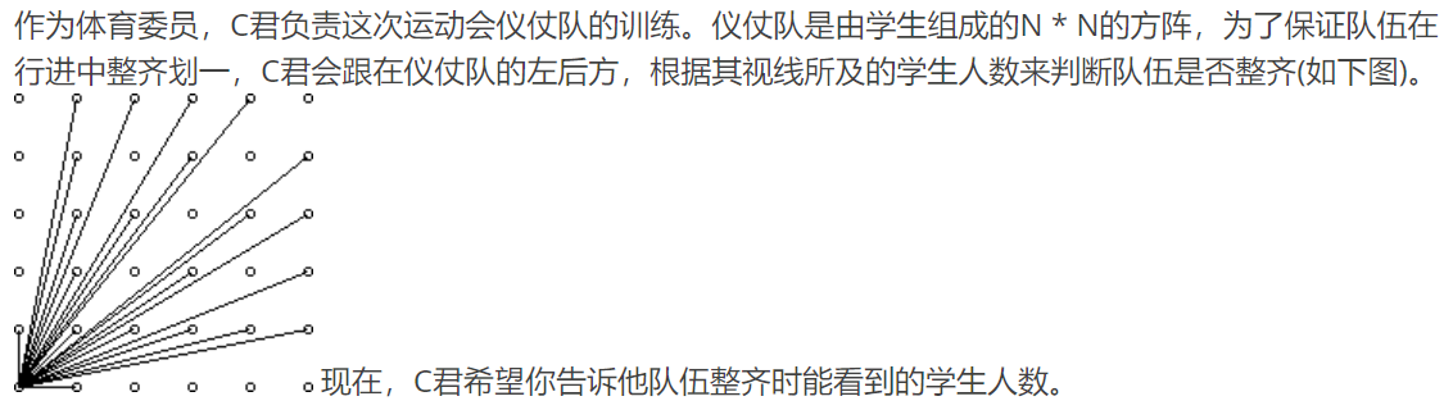
\includegraphics[width=0.7\textwidth]{images/img1.png}
    \end{figure}
  \end{block}

  \pause 
  \begin{exampleblock}{题解}
    \begin{itemize}
      \item 什么时候一个人会被另一个人挡住?
      \pause 
      \item 假设俩人坐标为$(x_1,y_1)$,$(x_2,y_2)$,$x_1\leq x_2$
      \item 显然当且仅当$\frac{y_1}{x_1}=\frac{y_2}{x_2}$时$2$会被$1$挡住
      \pause
      \item 只考虑$y<x$的部分,可得第$i$列只有$\varphi(i)$个人没被挡住,即可被看见
      \pause 
      \item 所以$ans =2*(\sum\limits_{i=1}^n\varphi(i))+1$
    \end{itemize}
  \end{exampleblock}
\end{frame}

\subsection{费马小定理}
\begin{frame}[fragile]{费马小定理}
  \begin{theorem}[费马小定理]
    若 $p$ 为素数,$\gcd(a, p) = 1$,则 $a^{p - 1} \equiv 1 \pmod{p}$。\\
    另一个形式:对于任意整数 $a$,有 $a^p \equiv a \pmod{p}$。
  \end{theorem}
  \pause 
  \vspace{0.5cm}

  费马小定理常用于结合\textbf{快速幂}求解\textbf{乘法逆元}:
  $$
  a^{p-2}\cdot a \equiv 1 \pmod{p}, (\gcd(a,p)=1)
  $$

  \pause
  \vspace{0.5cm}
  \textbf{证明}:\sout{我有一个对这个命题的十分美妙的证明,这里空白太小,我写不下了。}
\end{frame}

\begin{frame}[fragile]{费马小定理}{证明}
  \begin{proof}
    设一个质数为 $p$,且$\gcd(a,p)=1$。\\
    构造一个序列:$A=\{1,2,3\dots,p-1\}$,这个序列有着这样一个性质:
    $$
    \prod_{i=1}^{n}\space A_i\equiv\prod_{i=1}^{n} (A_i\times a) \pmod p
    $$
    
    \pause 
    思路:反证法可证得$\forall i\neq j,A_i a\not\equiv A_ja \pmod{p}$
    \\ 那么$\{A_ia\}$将取到$1\sim p-1$内的所有值。
    
    \pause 
    $$
    \begin{aligned}
      & \prod_{i=1}^{n}(A_i\times a) &\equiv\prod_{i=1}^{n} A_i &\pmod{p}\\
      \Rightarrow & a^{p-1}\prod_{i=1}^{n} A_i &\equiv\prod_{i=1}^{n} A_i &\pmod{p}\\
      \Rightarrow & a^{p-1} &\equiv 1 &\pmod{p}
    \end{aligned}
    $$
  \end{proof}
\end{frame}

\subsection{欧拉定理}
\begin{frame}[fragile]{欧拉定理}
  \begin{theorem}[欧拉定理]
    若 $\gcd(a, m) = 1$,则 $a^{\varphi(m)} \equiv 1 \pmod{m}$。
  \end{theorem}
  则当$m$为质数时,$\varphi(m)=m-1$,则可得$a^{m-1}\equiv 1 \pmod{m}$,即得到了费马小定理。
  
  \pause 
  \vspace{1.0cm}
  \textbf{证明}:\href{https://xdbirdie.github.io/2020/07/10/%E6%AC%A7%E6%8B%89%E5%AE%9A%E7%90%86%E4%B8%8E%E8%B4%B9%E9%A9%AC%E5%B0%8F%E5%AE%9A%E7%90%86/}{欧拉定理与费马小定理及证明}
\end{frame}

\begin{frame}[fragile]{拓展欧拉定理}
  欧拉定理只能在$\gcd(a,p)=1$时使用,限制很大。
  \pause
  \begin{theorem}[拓展欧拉定理]
    \begin{equation*}
      a^{b} \equiv\left\{\begin{array}{ll}
      a^{b \bmod \varphi(p)}, & \operatorname{gcd}(a, p)=1 \\
      a^{b}, & \operatorname{gcd}(a, p) \neq 1, b<\varphi(p) \quad(\bmod p) \\
      a^{b \bmod \varphi(p)+\varphi(p)}, & \operatorname{gcd}(a, p) \neq 1, b \geq \varphi(p)
      \end{array}\right.
    \end{equation*}
  \end{theorem}

  \pause 
  \vspace{0.3cm}
  完美满足所有情况,非常好用。\sout{(虽然我没怎么用过)}
  
  \pause
  \vspace{0.3cm}
  \textbf{证明}:\sout{太长了我写不下}\hspace{0.3cm} \sout{我不会}

  \pause 
  \vspace{0.3cm}
  常用于\textbf{欧拉降幂}。

\end{frame}

\begin{frame}[fragile]{拓展欧拉定理}{例题}
  \textbf{题目链接}:\href{https://acm.xidian.edu.cn/problem.php?id=1066}{P1066 A\^B\%P - XDOJ}
  \begin{block}{题目描述}
    求解:
    $$
    (\dots ((A^{B_0})^{B_1})\dots)^{B_{n-1}}\bmod{P}
    $$
    其中,$B_i=B_{i-1}^2-1(i>0)$,$P=1e9+7$。\\
    数据范围:$0<A<2^{31},0\le n\le 1e5,1<B_0<2^{31}$
  \end{block}
  \pause
  \begin{exampleblock}{题解}
    \begin{itemize}
      \item 即求$A^{\sum\limits_{i=0}^{n-1}B_i}\bmod{p}$,但是$B_i$是指数级增加,无法直接求出
      \pause 
      \item 显然\textbf{欧拉降幂},考虑适用条件
      \item $P=1e9+7$是质数,所以要么$\gcd(A,P)=1$,要么$P|A$
      \pause 
      \item 显然二者条件下,$A^{x}\equiv A^{x\bmod \varphi(P)} \pmod{P}$均成立
      \item 所以先求出$\sum\limits_{i=0}^{n-1}B_i\bmod{\varphi(P)}\;\;\;\;(\varphi(P)=P-1)$即可。
    \end{itemize}
  \end{exampleblock}
\end{frame}

% 乘法逆元
\section{乘法逆元}
\subsection{简介}
\begin{frame}[fragile]{乘法逆元}{简介}
  \textbf{乘法逆元}:如果一个线性同余方程 $ax \equiv 1 \pmod p$,则 $x$ 称为 $a$ 在$\pmod{p}$意义下的逆元,记作 $a^{-1}$。\\
  
  \pause
  \vspace{0.5cm}
  \textbf{用处}:
  \begin{itemize}
    \item 求解$\frac{A}{B}\bmod{P}$
    \item 避免浮点运算,提高精度
    \item 某些题目的要求
  \end{itemize}
  
  \pause 
  \vspace{0.5cm}
  \textbf{求解}:
  \begin{itemize}
    \item 快速幂方法
    \item 拓展欧几里得方法
    \pause
    \item 依据个人喜好
  \end{itemize}

\end{frame}

\subsection{单个求解}
\begin{frame}[fragile]{乘法逆元}{求解单个}
  \textbf{快速幂}
  \begin{itemize}
    \item \textbf{事实}:
    $$
    \begin{aligned}
       &\;& a^{p-1} &\equiv& 1 \pmod p \\
      &\Rightarrow& a\cdot a^{p-2} &\equiv& 1 \pmod p \\ 
      &\Rightarrow& x &\equiv& a^{p-2} \pmod p
    \end{aligned}
    $$
    \pause 
    \item \textbf{算法实现}:
    \begin{lstlisting}
inline int qpow(long long a, int b) {
  int ans = 1;
  a = (a % p + p) % p;
  for (; b; b >>= 1) {
    if (b & 1) ans = (a * ans) % p;
    a = (a * a) % p;
  }
  return ans;
}
// int inv = qpow(a, p - 2);
    \end{lstlisting}
    \pause 
    \item 时间复杂度:$O(\log{n})$
  \end{itemize}
\end{frame}

\begin{frame}[fragile]{乘法逆元}{求解单个}
  \textbf{拓展欧几里得}:
  \begin{itemize}
    \item \textbf{事实}:
    $$
    \begin{aligned}
      ax\equiv 1 \pmod{p}\\
      ax=(-y)\cdot p+1\\
      \text{求解:}ax+py=1
    \end{aligned}
    $$

    \pause
    \item \textbf{算法实现}:
    \begin{lstlisting}
int exgcd(int a, int b, int& x, int& y) {
  if (b == 0) {
    x = 1, y = 0;
    return a;
  }
  int g = exgcd(b, a % b, y, x);
  y -= a / b * x;
  return g;
}
// exgcd(a, p, x, y);
// int inv = (x % p + p) % p;
  \end{lstlisting}

  \pause 
  \item 时间复杂度:$O(\log{n})$
\end{itemize}
\end{frame}

\subsection{多个求解}
\begin{frame}[fragile]{乘法逆元}{求解$1\sim n$}
  线性时间复杂度求出 $1,2,...,n$ 中每个数关于 $p$ 的逆元。
  
  \pause 
  \begin{proof}
    \textbf{事实}:$\forall p \in \Z,\space 1 \times 1 \equiv 1 \pmod p$恒成立,即$\pmod{p}$意义下$1^{-1}=1$。\\
    
    \pause 
    \vspace{0.1cm}
    \textbf{思路}:通过$1\sim i-1$的逆元在$O(1)$的复杂度下求解$i^{-1}$。\\
    
    \pause 
    \vspace{0.1cm}
    设:
    $$
    k = \lfloor \frac{p}{i} \rfloor, \space j = p \bmod i, \space\text{则}p = ki + j
    $$
    
    \pause 
    我们有:
    $$
    \begin{aligned}
      &p=ki+j &\equiv& 0 &\pmod p&\\
      \pause 
      &ki\cdot{i^{-1}j^{-1}}+j\cdot{i^{-1}j^{-1}} &\equiv& 0\cdot{i^{-1}j^{-1}} &\pmod{p}& \\
      &k\cdot{j^{-1}}+i^{-1} &\equiv& 0 &\pmod{p}& \\
      \pause
      &i^{-1} &\equiv& -k\cdot{j^{-1}} &\pmod{p}& \\
      &i^{-1} &\equiv& -\lfloor \frac{p}{i} \rfloor \cdot j^{-1} &\pmod{p}&
    \end{aligned}
    $$
  \end{proof}
\end{frame} 

% 莫比乌斯反演
\section{莫比乌斯反演}
\subsection{数论分块}
\begin{frame}[fragile]{数论分块}
  \begin{lemma}
    $$
      \forall a,b,c\in\mathbb{Z},\left\lfloor\frac{a}{bc}\right\rfloor=\left\lfloor\frac{\left\lfloor\frac{a}{b}\right\rfloor}{c}\right\rfloor
    $$
  \end{lemma}

  \pause 
  \begin{proof}
    $$
    \begin{aligned}
      &\frac{a}{b}=\left\lfloor\frac{a}{b}\right\rfloor+r(0\leq r<1)\\
      \implies
      &\left\lfloor\frac{a}{bc}\right\rfloor
      =\left\lfloor\frac{a}{b}\cdot\frac{1}{c}\right\rfloor
      =\left\lfloor \frac{1}{c}\left(\left\lfloor\frac{a}{b}\right\rfloor+r\right)\right\rfloor
      =\left\lfloor \frac{\left\lfloor\frac{a}{b}\right\rfloor}{c} +\frac{r}{c}\right\rfloor
      =\left\lfloor \frac{\left\lfloor\frac{a}{b}\right\rfloor}{c}\right\rfloor\\
    \end{aligned}
    $$
  \end{proof}

  \pause 
  \begin{lemma}
    $$
    \forall n \in \mathbb{N}_{+},  \left|\left\{ \lfloor \frac{n}{d} \rfloor \mid d \in \mathbb{N}_{+},d\leq n \right\}\right| \leq \lfloor 2\sqrt{n} \rfloor
    $$
    $|V|$ 表示集合 $V$ 的元素个数。
  \end{lemma}
\end{frame}

\begin{frame}[fragile]{数论分块}{简介}
  求解类似于$\sum\limits_{i=1}^{n}f(\lfloor \frac{n}{i} \rfloor)$的式子。(假设$f(x)$可以$O(1)$求出)
  \begin{itemize}
    \item 直接求和,时间复杂度为$O(n)$,可通过数据约为$n\leq 1e8$。
    \item 事实上,$\lfloor \frac{n}{i} \rfloor$只有$O(\sqrt{n})$种,能否简化求和次数?
  \end{itemize}

  \pause 
  \vspace{0.3cm}
  对于任意一个 $i(i\leq n)$,我们需要找到一个最大的 $j(i\leq j\leq n)$,使得:
  $$
    \left\lfloor\frac{n}{i}\right\rfloor = \left\lfloor\frac{n}{j}\right\rfloor
  $$
  可得:
  \begin{center}
    $j=\left\lfloor\frac{n}{\left\lfloor\frac{n}{i}\right\rfloor}\right\rfloor$
  \end{center}
\end{frame}

\begin{frame}[fragile]{数论分块}{证明}
  \begin{proof} 
    $$
    \begin{aligned}
      &\left\lfloor\frac{n}{i}\right\rfloor \leq \frac{n}{i}\\
      \implies
      &\left\lfloor\frac{n}{ \left\lfloor\frac{n}{i}\right\rfloor }\right\rfloor
      \geq \left\lfloor\frac{n}{ \frac{n}{i} }\right\rfloor
      = \left\lfloor i \right\rfloor=i \\
      \implies
      &i\leq \left\lfloor\frac{n}{ \left\lfloor\frac{n}{i}\right\rfloor }\right\rfloor=j
    \end{aligned}
    $$
  \end{proof}
  
  \pause 
  \begin{itemize}
    \item \textbf{基本使用}:
    \begin{lstlisting}
for (int l = 1, r; l <= n; l = r + 1) {
  int t = n / l;
  r = n / t;
  // ... 若 l <= i <= r,那么 n / i == t 为真
}
    \end{lstlisting}
  \end{itemize}
\end{frame}

\begin{frame}[fragile]{数论分块}{例题}
  \textbf{题目链接}:\href{https://www.luogu.com.cn/problem/P2261}{P2261 [CQOI2007]余数求和 - 洛谷}
  \begin{block}{题目描述}
    给定正整数$n$和$k$,求解:
    $$
      G(n,k)=\sum\limits_{i=1}^n k \bmod{i}
    $$
    数据范围:$1\leq n, k\leq 10^9$
  \end{block}
  
  \pause
  \begin{exampleblock}{题解}
    \begin{itemize}
      \item 直接求和,$O(n)$时间复杂度会TLE。
      \pause
      \item 转化为整除形式,然后数论分块:
      $$
        \begin{aligned}
          ans &= \sum_{i=1}^n(k\bmod i) 
               = \sum_{i=1}^nk-i\left\lfloor\frac{k}{i}\right\rfloor 
               = n\cdot k - \sum_{i=1}^{\min(n,k)} i\left\lfloor\frac{k}{i}\right\rfloor
        \end{aligned}
      $$
    \end{itemize}
  \end{exampleblock}
\end{frame}

\begin{frame}[fragile]{数论分块}{例题}
  
  \begin{itemize}
    \item \textbf{算法实现}:
      \begin{lstlisting}
#include<iostream>
using namespace std;

inline long long sum(long long i, long long j){
    return (j * (j + 1) / 2 - i * (i - 1) / 2);
}

int main(){
    long long n, k, ans;
    cin >> n >> k;
    ans = n * k;
    for (long long i = 1, j; i <= k && i <= n; i = j + 1){
        long long t = k / i;
        j = min(k / t, n);
        ans -= t * sum(i, j);
    }
    cout << ans ;
    return 0;
}
    \end{lstlisting}
  \end{itemize}
\end{frame}

\begin{frame}[fragile]{数论分块}{例题}
  \textbf{题目推荐}:
  \begin{itemize}
    \item \href{https://www.luogu.com.cn/problem/P2261}{P2261 [CQOI2007]余数求和 - 洛谷}
    \item \href{https://www.luogu.com.cn/problem/P2260}{P2260 [清华集训2012]模积和 - 洛谷}
    \item \href{https://codeforces.com/gym/101485/attachments}{Debugging - Codeforces}
  \end{itemize}
\end{frame}

% Questions
\section{结束}
\begin{frame}
\begin{center} {\bfseries \Huge Questions?} \end{center}
\end{frame}


\end{document}